\documentclass{article}
% ready for submission
\usepackage[final]{neurips_2023}

% Language setting
% Replace `english' with e.g. `spanish' to change the document language
\usepackage[english]{babel}

% Set page size and margins
% Replace `letterpaper' with `a4paper' for UK/EU standard size
% \usepackage[letterpaper,top=2cm,bottom=2cm,left=3cm,right=3cm,marginparwidth=1.75cm]{geometry}

% Useful packages
\usepackage{amsmath}
\usepackage{graphicx}
\usepackage[colorlinks, linkcolor = black, citecolor=red, urlcolor=black]{hyperref}

\usepackage[utf8]{inputenc} % allow utf-8 input
\usepackage[T1]{fontenc}    % use 8-bit T1 fonts
\usepackage{url}            % simple URL typesetting
\usepackage{booktabs}       % professional-quality tables
\usepackage{amsfonts}       % blackboard math symbols
\usepackage{nicefrac}       % compact symbols for 1/2, etc.
\usepackage{microtype}      % microtypography
\usepackage{xcolor}         % colors
\usepackage{hyperref}       % emails
\usepackage{marvosym}
\usepackage{float}          % figures placing

\title{Binary Image Classification on Camera Trap Data for Detecting Sarcoptic Mange in Coyotes
}

\author{
  Steven Tang \\
  Department of Computing Science \\
  University of Alberta \\
  \href{mailto: stang5@ualberta.ca}{\texttt{stang5@ualberta.ca}} \\
  \And 
  Akemi Izuko \\
  Department of Computing Science \\
  University of Alberta \\
  \href{mailto: izuko@ualberta.ca}{\texttt{izuko@ualberta.ca}} \\
  \And 
  Tim Van Maren \\
  Department of Computing Science \\
  University of Alberta \\
  \href{mailto: vanmaren@ualberta.ca}{\texttt{vanmaren@ualberta.ca}} \\
  \And 
  Yongshan Yu \\
  Department of Computing Science \\
  University of Alberta \\
  \href{mailto: yongshan@ualberta.ca}{\texttt{yongshan@ualberta.ca}} \\
  \And
  Moyinoluwa Famobiwo \\
  Department of Computing Science \\
  University of Alberta \\
  \href{mailto: famobiwo@ualberta.ca}{\texttt{famobiwo@ualberta.ca}} \\
  \And
  Sanad Masannat \\
  Department of Computing Science \\
  University of Alberta \\
  \href{mailto: sanad@ualberta.ca}{\texttt{sanad@ualberta.ca}} \\
}


\begin{document}
\maketitle


\begin{abstract}
In recent decades, \textbf{C}onvolutional \textbf{N}eural \textbf{N}etworks (CNNs) and \textbf{M}achine \textbf{L}earning (ML) have made remarkable progress in the field of Computer Vision. This study explores the application of these technologies to a novel domain: detecting sarcoptic mange in coyotes using camera trap data. We examine their strengths and weaknesses in addressing the unique challenges posed by this specific domain, providing insights into the difficulties of using camera trap images for wildlife skin disease detection, and suggesting potential solutions to overcome these challenges. We propose a Residual Neural Network model and data preprocessing steps, which result in an 18\% improvement on our expected cost evaluation metric when compared with simple baseline models, while also achieving a recall of 71\% when evaluated using 5-fold cross validation. We additionally provide valuable insights regarding further application of ML in the domain of camera trap data analysis, and emphasize the importance of developing more robust models tailored to similar domains.
\end{abstract}
%TODO: check final values

\section{Background}
Detecting sarcoptic mange in coyotes (\textit{Canis latrans}) is a critical task for wildlife conservation and ecology. Sarcoptic mange is the predominant form of mange in coyotes, leading to severe inflammation and symptoms such as fur loss, darkened skin, self-inflicted wounds due to intense irritation \cite{Murray2021} and in worse cases, blindness and death. Since mange-infected coyotes are usually secluded, upon discovery their condition may have progressed past the possibility of recovery \cite{C469Meeting}. Therefore, developing an efficient detection method is essential for timely intervention and treatment.

Motivated by this problem, we propose an image classifier based on camera trap data to detect mange-infected coyotes. Given that the labels in our dataset are provided by human expert annotators, the best model can learn to match human experts on whether mange is detected or not. Camera trapping - widely employed in wildlife observation - captures consecutive images upon detecting motion, with approximately 30-second intervals between them \cite{C469Meeting}. Camera traps provide valuable data for detecting mange in coyotes; however, the quality of the acquired data poses challenges to our research.

As shown in Figure \ref{fig:fig1}, the trained image classifier must detect mange in coyotes within images with characteristics that may pose challenges to learning using CNNs.
In addition, the limited variety of labeled training data available for this task exacerbates these challenges. Several hundred images are taken from the same camera, and the severe imbalance caused by the CumberlandA dataset contributes to the difficulty. To address these issues, we explore various image processing techniques designed to improve the neural network's performance in detecting mange under a range of conditions.

\begin{figure}[h]
\centering
% \vspace{-0.3cm}
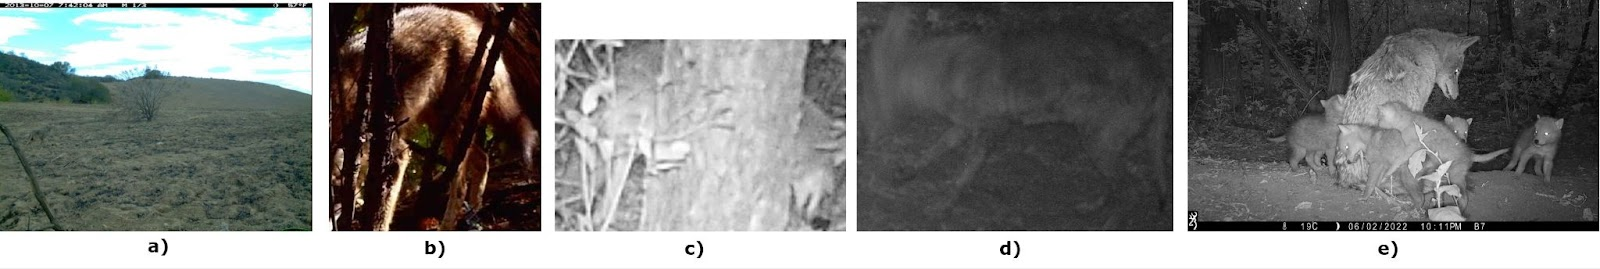
\includegraphics[width=1.0\textwidth]{fig1.jpeg}
\caption{\label{fig:fig1}Examples of challenging images from our datasets: \textbf{a)} The coyote camouflages with its surroundings. \textbf{b)} Image with only a portion of the coyote visible. \textbf{c)} Image captured at night with poor illumination. \textbf{d)} Image blurry due to coyote motion. \textbf{e)} Multiple close-up coyotes in one image.}
\end{figure}
% \vspace{-1.3cm}
By employing these techniques, we aim to develop an image classification model capable of automatically detecting mange in coyotes. This will significantly improve the efficiency of mange detection, alleviate the workload of ecologists and wildlife conservationists, and provide robust support for timely intervention and treatment of mange. 

We proceed with the task description in Section
\ref{sec:task description} to
establish the context of our study. Section \ref{sec:lit review} discusses prior research in animal skin disease classification as well as research relying on camera trap data for wildlife inference. Section \ref{sec:methods} delves into our methodology, covering
the various approaches and techniques we employed in pursuit of our objectives. Section \ref{sec:evaluation} then outlines the metrics and evaluation methods used to assess our
model's performance, providing a quantitative understanding of our results. Section \ref{sec:results} presents the results of our empirical study.
Section \ref{sec:discussion} discusses our results, addressing limitations and exploring
potential avenues for future work.

\section{Task Description} \label{sec:task description}

Our task is to identify sarcoptic mange in coyotes from camera trap images by developing a binary classification algorithm. This task is suited to a vision-based machine learning approach as there are visual cues in mange-infected coyotes such as visible hair loss \cite{Murray2021}. To illustrate the task more concretely, Figure 2 shows a simple example: given an input image of a coyote captured by a camera trap, our model makes a prediction and labels the image as either "mange detected" or "mange not detected" based on its previously learned knowledge. The model is to be learned from training data, and we have been advised by our domain experts to maintain cost-sensitive learning, with false negatives being penalized at 5 times the cost of false positives.

Our labeled dataset consists of 14,760 images from camera traps in North America; specifically in Toronto, Chicago, and Edmonton. In the dataset, 1,929 (13\%) images are labeled as "mange detected." Human expert annotators determined the labels, which are provided in CSV files alongside the images. The data set also includes timestamps and approximate locations for each image. 

\begin{figure}[ht]
\centering
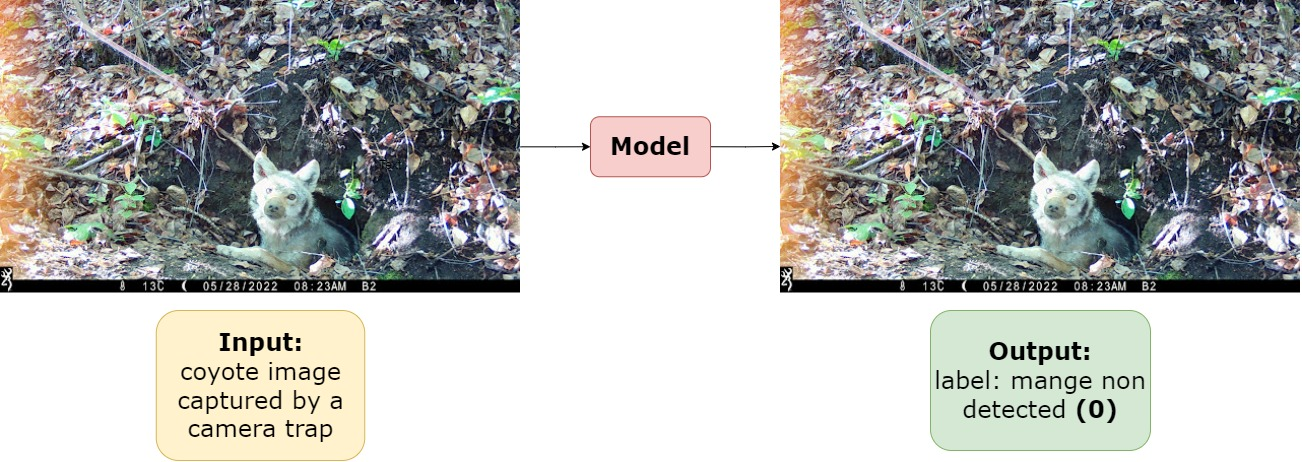
\includegraphics[width=1.0\textwidth]{fig2.jpg}
%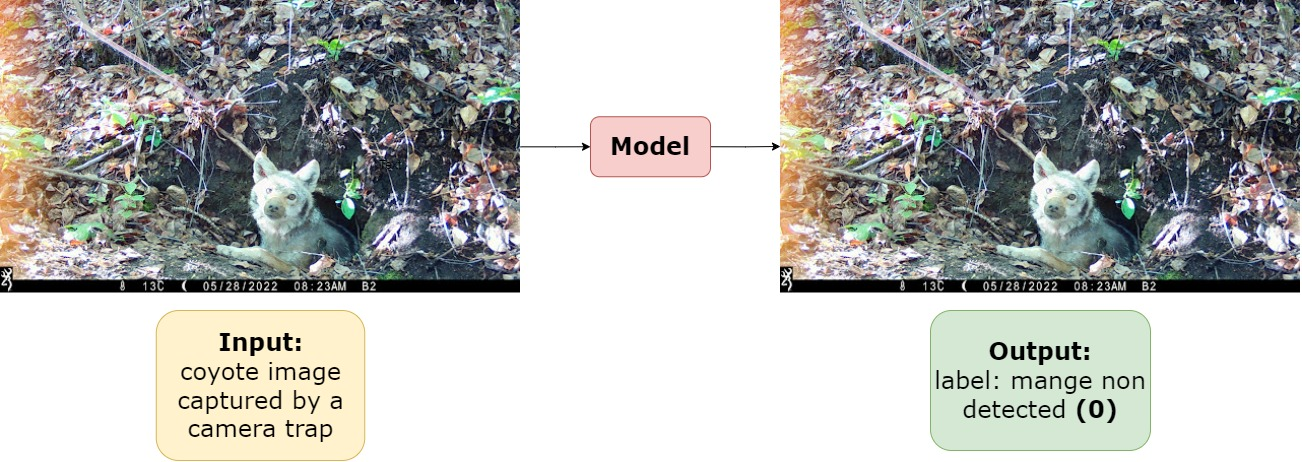
\includegraphics[scale=0.2]{fig2.jpg}
\caption{\label{fig:fig2}A simple example of our task: the input is a coyote image captured by a camera trap, and the desired output is a single class label indicating mange not detected (0) or mange detected (1).}
\end{figure}

Considering the distribution described in the previous paragraph, the dataset for this study exhibits an imbalanced class distribution. This imbalance can be attributed to the relatively low occurrence of mange in wild coyotes, which results in a substantially smaller number of positive cases (mange detected) compared to negative cases (mange not detected) within the dataset. Moreover, as shown in Figure \ref{fig:output} in the Appendix, variations in the number of images captured by camera traps at each location contribute to an uneven location distribution within the dataset.

\section{Related Works} 
\label{sec:lit review}
Animal skin disease classifiers that have shown success tend to use pictures taken within very close range of the animal, with no extraneous background details. These pictures also tend to have very high resolutions, making it easier for the model to discern between features in the image. An example of this is presented by Hwang \textit{et al}. \cite{Hwang2022}, as they were able to achieve up to 89\% accuracy using deep learning methods, but used images of pet dogs taken on mobile devices within centimeters of the dog’s skin. Some of the methods used within this study, such as data augmentation and the use of Residual Neural Networks, were suitable for our approach due to the common objective of image classification. 
However, their results are not directly comparable with ours as their training data is exceedingly different from the data obtained from camera traps.

The use of camera trapping within ecological research is widespread, and ML methods are successfully being utilized to take advantage of the data becoming available. However, despite ML's success in this domain and in classifying skin diseases in domestic animals, the research within our specific domain, which combines both of the aforementioned domains, is very limited. 
Object detection models have been successfully used to process camera trap data, and one notable model that has been developed specifically for this task is MegaDetector, which has achieved 96.6\% accuracy in animal image detection, with a precision of 82\% and recall of 92\% at a confidence level of 90\% \cite{Fennell2022}. As MegaDetector has been developed with the aim of accelerating ecological research by automatically identifying bounding boxes of animals, we found it suitable for use in this study, and details of its use are expanded upon in Section \ref{sec:methods}.

\section{Methods} \label{sec:methods}

\subsection{MegaDetector}
In our attempt to classify sarcoptic mange, we decided to first perform preprocessing on the data before employing any models. As we noticed poor performance when working directly with the data without any preprocessing, we hypothesized that one of the critical challenges to our research problem was the presence of a largely extraneous background. The noise caused from this could potentially confuse the models, particularly learning the distribution of mange in the training set for specific backgrounds. To address this issue, we decided to crop the images to emphasize the coyotes and minimize the influence of the background.

To crop the images, we used MegaDetector, an AI model trained to detect objects including animals in camera trap images \cite{Fennell2022, beery2019efficient}. Developed by conservation biologists, MegaDetector streamlines the process of reviewing camera trap images by identifying objects of interest without classifying species. It helps to extract relevant information from the images, reducing noise in the image by quickly removing the majority of the background in most pictures and emphasizing the coyote itself.

Figure 3 provides a simple example of the preprocessing on our data. MegaDetector identified the bounding box around the coyotes in each image. After obtaining these bounding boxes, we cropped the images to these boxes. This was done to encourage the model to concentrate on what our domain experts believed to be the essential features for mange detection.

\begin{figure}[H]
\centering
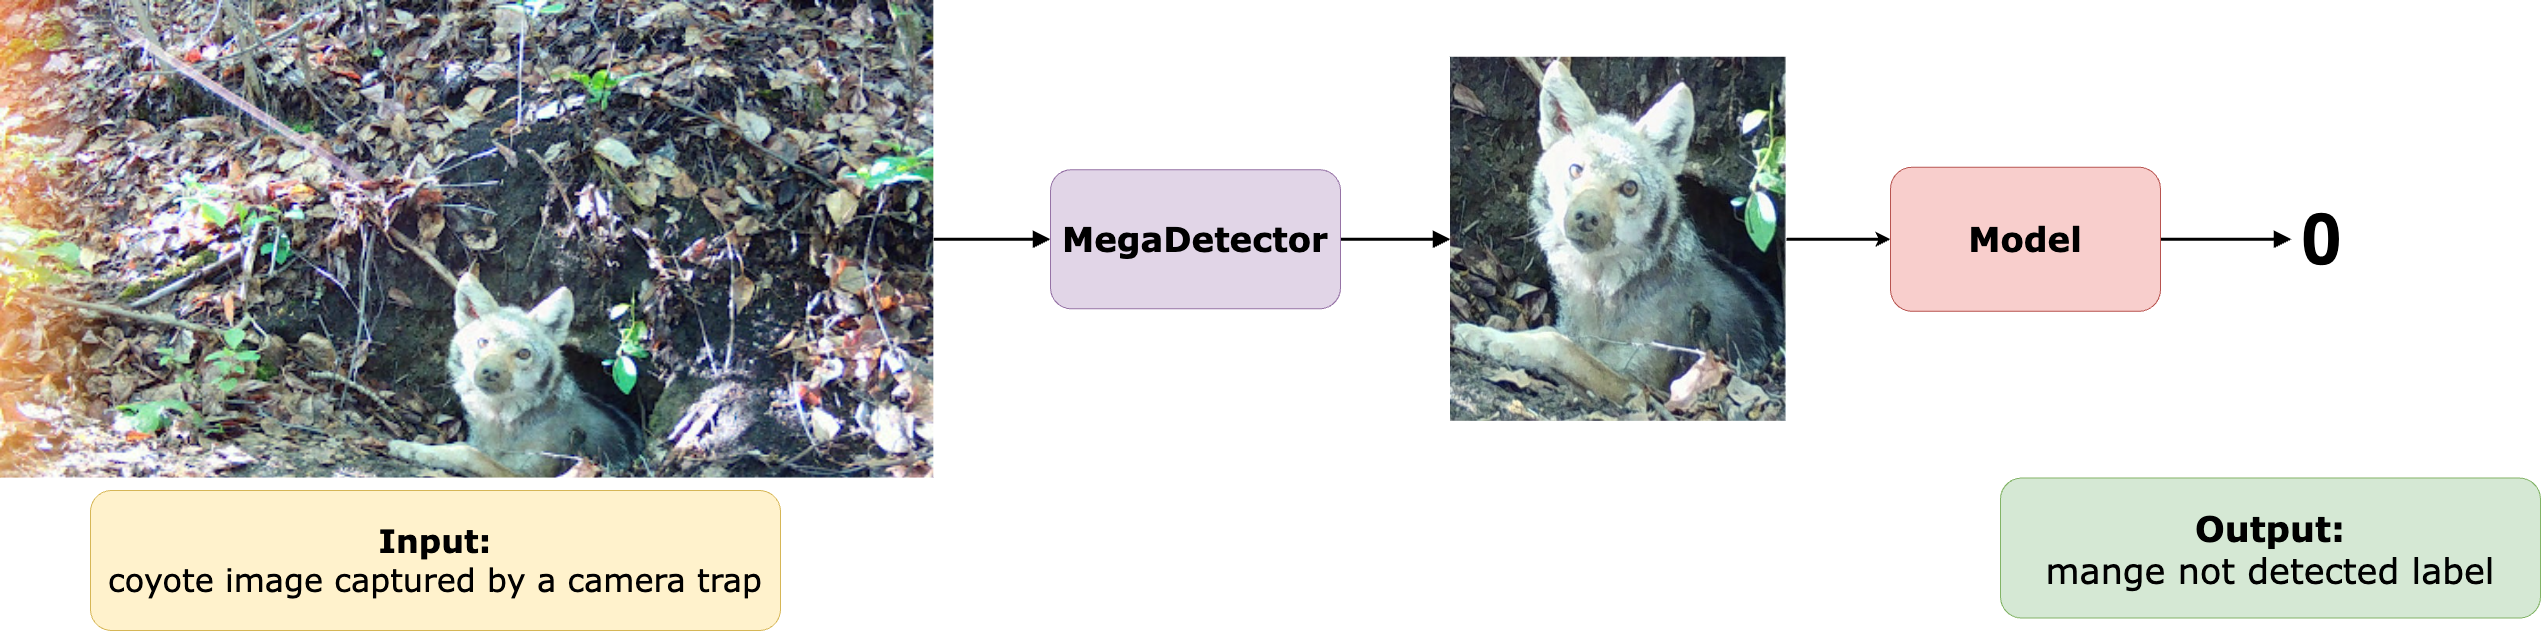
\includegraphics[width=1.0\textwidth]{fig3.png}
\caption{\label{fig:fig3}An example of data preprocessing using MegaDetector. The original camera trap image of a coyote with extraneous background information (left) is processed by MegaDetector, which identifies the bounding box around the coyote in the image. The cropped image based on the bounding box emphasizes the coyote and minimizes the influence of the background (right).}
\end{figure}

Before cropping our entire dataset, we used human labellers to evaluate how often these key features for mange detection were contained in MegaDetector’s bounding box. We found 82\% of bounding boxes for images with tails were able to capture over 50\% of the original tail within their bounds.

\subsection{Data Augmentation}
Data augmentation is a process in which we include slightly modified images during training. This can improve the generalization capabilities of deep learning models \cite{Shorten2019} by adding inductive bias to our model, which encourages it to be invariant to certain properties like rotation, scaling, and variations in brightness. 
We note that the CNN architecture is already translationally invariant, and thus there is no need to augment for this. 
Some common data augmentation methods include: horizontal/vertical flipping, rotation, gaussian blurring, random cropping, noise insertion and color jittering. However, since different augmentations affect generalization differently, we experimented with multiple data augmentation techniques to see which ones presented the most significant improvement to generalization. On a subset containing 511 images from Chicago, we found that applying horizontal flipping, rotation, and gaussian blurring resulted in improved generalization. We found data augmentation promising and evaluated its use in our final model.

\subsection{Data Programming} 
In addition to the labeled coyote images, we found an additional 40,285 unlabeled coyote camera trap images \cite{DBLP:BeeryHP18}. 
%Despite the prohibitive cost of labeling such a massive amount of images, the prospect of improved performance from training on the unlabeled data was worth exploring. 
Semi-supervised learning approaches were suitable here to take advantage of this additional data. Specifically, we considered data programming, as shown by Ratner \textit{et al.} \cite{ratner2017data}, which uses a heuristic function 
% developed from the process of labeling , as described by the domain experts,
to “weakly” label the data. 
%“Weak” labels are much noisier than their hand-labeled counterparts, though the sheer quantity of weak labels has been shown to help reduce the noise present in the dataset as a whole.
Our domain experts provided the process they use for checking coyote images for mange \cite{C469Meeting}:
\begin{enumerate}
    \item If available, look at the thickness of the tail. This is one of the first signs of mange, as the tail's length-to-width ratio is quite different when comparing a healthy tail and a tail with lost fur.
    \item Look for bald patches of fur on the coyote’s back.
\end{enumerate}

Heuristic functions attempting to encode the above process were challenging due to  noise.
For tail analysis, our functions wrongly labeled almost all images as containing a mange-infected tail, due to picking up the twigs and branches in the background instead of the tail. 
%Furthermore, when we labeled a random subset of our data, we found only 61\% of the images contained over 50\% of the coyote’s tail. 
For fur analysis, we considered texture-based computer vision. However, as found by other studies \cite{rs15010170}, most of our images were too low resolution to accurately detect differences in fur texture. Ultimately, the domain-knowledge encoding resulted in largely random labeling, so we were unable to apply this approach on either dataset.

\subsection{Tabular Features}
We ran experiments including tabular features such as the hour of the day, the month and the year in which the picture was taken, whether the image was in gray scale or full color, and the longitude and latitude of the camera trap. Color affects the expert's ability to classify mange, the time of day at which the coyote was spotted may be correlated with the behaviour of a mange-infected coyote, and the time of year and location may be correlated with higher occurrences of mange \cite{C469Meeting}, 
thus we included these tabular features with our data in hopes of improving the classifier's accuracy.
To do this, we concatenated the features with the image backbone output and learned a linear weighting.

\subsection{Weighted Binary Cross Entropy Loss}

We used \textbf{w}eighted \textbf{B}inary \textbf{C}ross \textbf{E}ntropy (wBCE) as our loss function. wBCE modifies Binary Cross Entropy (BCE) loss with a parameter $p$ such that values of $p > 1$ punish false negatives more than false positives \cite{Ozdemir2020}. We selected this loss to account for class imbalance in our dataset and the unbalanced cost of false negatives and false positives in our evaluation criteria.
  \begin{equation}
  \ell(x, y) = \frac{1}{N}\sum_{i = 1}^N p \cdot y_i \cdot \log f(x_i)
+ (1 - y_i) \cdot \log (1 - f(x_i)),
\end{equation}
where $f(x_i)$ is the output of our model for the $i$-th sample with input $x_i$
and label $y_i$, and $p$ is the weight of positive examples.
We set $p$ to be 5 times the ratio of the number of "no mange detected" samples to the
number of "mange detected" samples in the training set to adjust for the class
imbalance in our dataset; we multiply by 5 as the cost of false negatives is 5 times more than the cost of false positives in our expected cost evaluation criteria.
\begin{equation}
  p = 5 \cdot \frac{N_{\text{no mange detected}}}{N_{\text{mange detected}}}
\end{equation}

 We also tried other loss functions including: Expected Cost, Macro Soft F$_\beta$ \cite{lee2021surrogate}, and Surrogate F$_\beta$ \cite{lee2021surrogate}, but they did not perform as well as wBCE loss.

\subsection{Learning Rate Finder}
We decided to make use of a Learning Rate Finder to streamline tuning of the initial learning rate. Considering the computational resources and time needed to train a model on our data, exhaustively experimenting with various learning rates would not have been feasible. Instead, the Learning Rate Finder approximates the optimal learning rate on a small subset of the data by iterating linearly through settings and observing the loss produced. This process continues until the loss diverges or the maximum value is reached. The model then selects the learning rate where the steepest convergence began. This functions similarly to estimating minimum and maximum boundary values when using cyclical learning rates \cite{Smith:2017}.

Note that using a Learning Rate Finder to set an initial learning rate can only provide a reasonable estimate of an optimal setting \cite{Smith:2017}. In our experimentation, we found that this method did not perform well when using BCE loss, often selecting an initial learning rate greater than 0.1. However, the Learning Rate Finder seemed to perform well when used in conjunction with wBCE loss.

\subsection{Optimization}
We used Adam as our optimization algorithm. Kingma \textit{et al}.'s \cite{kingma2017adam} empirical results show that it works well in
practice and is favourable to other stochastic gradient optimization methods on an image classification problem. We used a learning rate scheduler to halve the learning rate after 4 epochs without improvement in validation loss. To prevent overfitting, we used early stopping after 5 epochs without improvement in validation loss.

\subsection{Transfer Learning}
Considering the %relatively small size 
challenges inherent to the lack of variety in our dataset, we decided to apply transfer learning to our task. Previous work in the area of camera trap image classification using deep learning has shown that the same level of accuracy achieved on a dataset of over a million images can be achieved on a far smaller subset of that dataset with the use of transfer learning \cite{Norouzzadeh2018}. Transfer learning works best when the base model was trained for a task very similar to our own \cite{Yosinski2014}. However, this technique can still improve generalization performance after significant tuning on a new task \cite{Yosinski2014}. 

\subsection{Models}

\subsubsection{Vision Transformers}
Given the recent successes of the transformer model \cite{vaswani2017attention} in the domain of language processing, computer vision research has quickly adopted the architecture \cite{dosovitskiy2021image}.  Visual attention models have shown promising results, particularly in image classification settings where the majority of the image is not relevant to the task, such as housing numbers on street-view data \cite{ba:2014}, and even with identifying leaf diseases \cite{Alshammari2022}. However, vision transformers models had high expected cost results and did not improve on our baselines. As our final evaluation metric was expected cost, we chose to not pursue transformer methods any further.

\subsubsection{YOLO and DenseNet}
The You Only Look Once (YOLO) family of models are CNN-based object detection models which predict bounding boxes for objects of interest \cite{RedmonDGF15}. They have been shown by Wang \textit{et al}. \cite{WANG2022100646}, who used YOLOv5 for accurate detection of dairy cow mastitis, to locate the key parts of the cow with an average accuracy of 96.1\%, leading to a detection accuracy of 85.71\%.
We were motivated to use the YOLOv8 model as our base model for transfer learning, seeing as a model architecture designed for object detection might be better able to focus on the coyote within the image and detect the key features for mange detection. 
DenseNets are deep neural networks which use feed-forward connections between each layer, strengthening feature propagation and reducing the number of training parameters \cite{HuangLW16a}. Hwang \textit{et al}. \cite{Hwang2022} had success using DenseNet121 for the classification of dog skin diseases, motivating its use for our task. However, neither the YOLOv8 nor the DenseNet121 model had lower expected cost when compared with the ResNet models.

\subsubsection{Residual Neural Networks}
The Residual Neural Network (ResNet) models are useful for image classification and were developed to solve the problem of gradient degradation which arises when training deep neural networks \cite{HeZRS15}. ResNets accomplish this by learning residual representations and using skip connections between layers. For our task, we
chose to use the ResNet architecture for transfer learning and 
conducted experiments using the ResNet18, ResNet34, and ResNet50 models. We conducted experiments using the deeper ResNet architectures as well, but they did not perform better than ResNet50.


\section{Evaluation} \label{sec:evaluation}

For evaluation, we adopted 5-fold cross-validation to estimate generalization performance \cite{Berrar2019, Schaffer1993}.
This approach involves dividing the data set into five folds.
In each iteration, one of the folds serves as the test set, and the remaining folds are combined with 80\% split as the training set and 20\% as the validation set. We use stratification to preserve the ratio of mange detected to mange not detected across folds. This procedure is repeated five times, and the overall generalization performance is assessed by averaging the results from all five iterations.

To prevent data leakage in cross-validation, we ensured that the test set did not include images nearly identical to those in the training set. We achieved this by partitioning the set of images into subsets based on location. All images within a subset were then assigned to only one of the training, validation, or testing sets. This separation ensures that our model is evaluated on its ability to generalize to unseen data based on the actual classification task, rather than memorizing a coyote repeated across several images.

There are two different costs in our evaluation, a false positive ($FP$) results in a detection of a healthy coyote as mangy, which results in a cost to the domain expert who has to filter it out manually. On the other hand, a false negative ($FN$) means that a coyote with mange is not detected and could potentially infect other coyotes.

For general understanding, we evaluated precision and recall. Precision is the proportion of coyotes with mange detected that actually have mange, and recall is the proportion of coyotes with mange that are detected.

\begin{equation}
  \text{Precision} = \frac{TP}{TP+FP} \qquad \text{Recall} = \frac{TP}{TP+FN}
\end{equation}

However, our primary evaluation metric was expected cost determined by our domain experts, which assessed the model's practical performance. In consultation with our domain expert, a false negative costs 5 times more than a false positive.

\begin{equation}
  EC_5 = \frac{5FN + FP}{N}
\end{equation}

Where $N$ is the total number of data samples. Note that a lower expected cost is better.

We calculate 95\% confidence intervals for all metrics by running cross validation 30 times and using the standard error of the results. We conduct hypothesis testing for expected cost between different models using one-tailed two-sample unequal variance t-tests to identify whether two models are statistically different with $\alpha = 0.05$. The null hypothesis is that the models A and B, have the same mean expected cost, $EC_{5A} = EC_{5B}$. The alternative hypothesis would be that one of the models has a lower expected cost than the other $EC_{5A} < EC_{5B}$.

\section{Results} \label{sec:results}

Our final model is a ResNet34 trained with weighted Binary Cross Entropy (wBCE) loss, transfer learning (TL), no MegaDetector cropping (MD), no data augmentation (DA), and no tabular features (TF). 
Table 1 compares the mean standard error of metrics obtained across different models.

For comparison, we report results of 3 baselines,
All Positive, which always predicts mange detected,
All Negative, which always predicts mange not detected, and 
Random, which predicts mange with a $50\%$ random chance.

\begin{figure}[H]
  \centering
  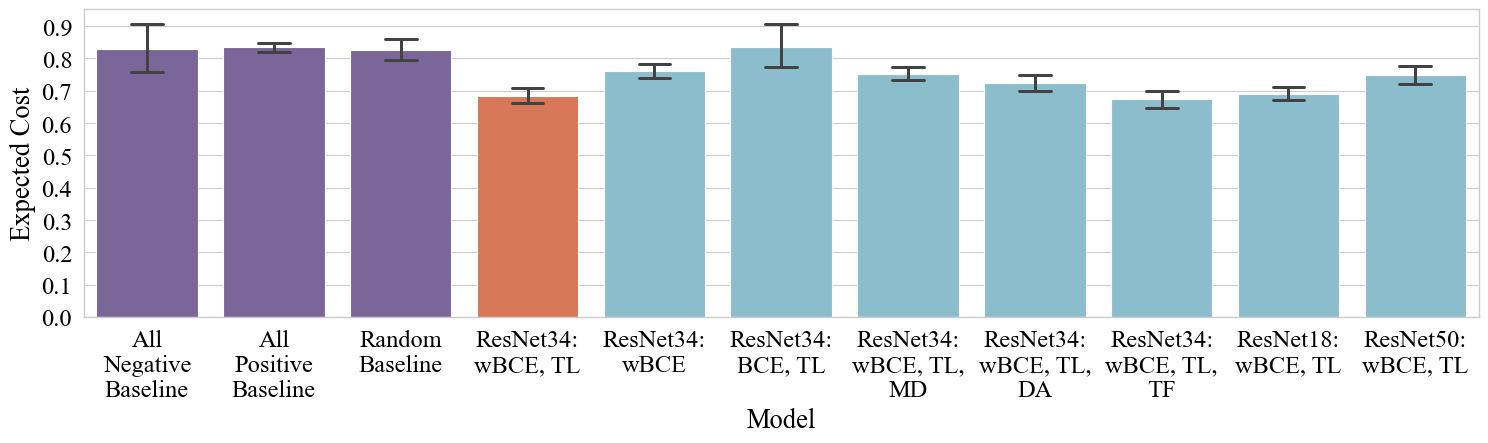
\includegraphics[width=\textwidth]{fig4.png}
  \caption{\label{fig:fig4}Comparison of Expected Cost between models with 95\% Confidence Intervals. 
  Purple: baselines; Red: our final model; Blue: other models we tried}
\end{figure}

With $\alpha = 0.05$, we can reject the null hypothesis, and accept the alternative hypothesis, that our model achieves a statistically significant lower mean expected cost than the All Negative ($p = 4 \times 10^{-4}$), All Positive ($p = 2 \times 10^{-13}$), and Random ($p = 3\times 10^{-9}$) baselines. 
Similarly, our final model achieves a statistically significant lower mean expected cost than models similar in all aspects except: trained with BCE ($p = 2 \times 10^{-4}$), without transfer learning ($p = 2\times10^{-5}$), with MegaDetector cropping ($p = 1 \times 10^{-4}$), with data augmentation ($p = 0.02$), and with ResNet50 ($p = 7 \times 10^{-4}$). There is no statistical difference between our final model and models similar in all aspects except: with tabular features ($p = 0.3$) and with ResNet18 ($p = 0.3$).

% todo evaluate for BCE and data augmentation and tabular features
% cropping vs ResNet18 vs ResNet50
% TODO: cut stuff until this table stops overflowing onto next page!
\begin{table}[ht!]
  \label{t1}
  \caption{Mean $\pm$ 95\% standard error of metrics obtained using 95\% confidence intervals on 30 repeated trials of 5-fold cross validation on entire dataset. Our final model is bolded. Abbreviations: weighted Binary Cross Entropy (wBCE), Transfer Learning (TL), MegaDetector cropping (MD), 
Data Augmentation (DA), Tabular Features (TF).}
  \centering
  \begin{tabular}{llll}
  \toprule

    \topfigrule
    Model     & Expected Cost     & Precision & Recall \\
    \midrule
    All Negative Baseline & $0.83 \pm 0.08$    & $0.00 \pm 0.00$ & $0.00 \pm 0.00$     \\
    All Positive Baseline & $0.83 \pm 0.02$    & $0.17 \pm 0.02$ & $1.00 \pm 0.00$     \\
    Random Baseline & $0.83 \pm 0.03$    & $0.17 \pm 0.02$ & $0.50 \pm 0.01$     \\
    \midrule
    \textbf{ResNet34: wBCE, TL} & $0.68 \pm 0.03$ & $0.20 \pm 0.02$ & $0.71 \pm 0.02$     \\
    \midrule
    ResNet34: BCE, TL & $0.84 \pm 0.07$ & $0.11 \pm 0.04$ & $0.04 \pm 0.01$ \\
    ResNet34: wBCE & $0.76 \pm 0.02$ & $0.18 \pm 0.02$ & $0.72 \pm 0.02$     \\
    ResNet34: wBCE, TL, MD & $0.75 \pm 0.02$ & $0.18 \pm 0.02$ & $0.75 \pm 0.02$ \\
    ResNet34: wBCE, TL, DA & $0.72 \pm 0.03$ & $0.19 \pm 0.02$ & $0.60 \pm 0.04$ \\
    ResNet34: wBCE, TL, TF & $0.67 \pm 0.03$ & $0.21 \pm 0.02$ & $0.70 \pm 0.03$ \\
    ResNet18: wBCE, TL & $0.69 \pm 0.02$ & $0.20 \pm 0.02$ & $0.73 \pm 0.03$     \\
    ResNet50: wBCE, TL & $0.75 \pm 0.03$ & $0.18 \pm 0.02$ & $0.70 \pm 0.03$     \\
    \bottomrule \\
  \end{tabular}
\end{table}

% TODO: Possibly appendix toronto results...

\section{Discussion} \label{sec:discussion}
In our study, we found that models trained using wBCE loss demonstrated better performance than those utilizing BCE loss. This can be attributed to wBCE's capability to handle class and cost imbalance effectively. Additionally, transfer learning contributed to a statistically significant reduction in expected cost.

Nevertheless, when using images cropped by MegaDetector, the models consistently showed higher expected costs. Upon closer inspection, it was evident that the models focused more on the image padding rather than the actual content. Including tabular features did not lead to significant improvements, and therefore, they were not incorporated into the final model.

Comparing the performances of ResNet18, ResNet34, ResNet50, and visual transformers we observed that the ResNet18 and ResNet34 models yielded the lowest expected cost. We believe that the ResNet50 model and vision transformers experienced overfitting due to their large number of parameters, resulting in higher expected costs. There was no statistically significant difference between the ResNet18 and ResNet34 models, with $\alpha = 0.05$. 

Our final model outperformed the baselines, with an 18\% improvement in expected cost, achieving 20\% recall and 71\% precision. However, it is far from perfect and shows that determining an optimal model for this task will require further research.
 
\subsection{Future Work}
Given the comparative scarcity of labeled data and the difficulty associated with unsupervised learning in such noisy settings, we suggest further research consider co-learning \cite{Blum:1998} and other semi-supervised learning methods to take advantage of readily available unlabeled data.

\section{Conclusion}
In this paper, we examined the application of different neural network architectures towards the detection of sarcoptic mange in coyotes. We conducted empirical research using a range of models with previous success in image classification tasks, as well as different data preprocessing techniques, data augmentation methods, evaluation metrics, and hyperparameter tuning. 
Upon concluding our study, we found that the classifier with the lowest expected cost was a ResNet34 model trained with transfer learning, no data augmentation, no
cropping, and weighted Binary Cross Entropy Loss. Involvement in this study improved our understanding of the difficulties associated with applying machine learning methods to novel domains. 

\clearpage

\acksection{}
\label{sec:acknowledgements}
We would like to thank our domain experts Tiziana A. Gelmi Candusso, Sage
Raymond, Maureen Murray, and Mason Fidino, who provided us with the coyote
camera trap data and their expertise to guide us along this project. We
would also like to thank professor Russ Greiner and teaching assistant Thang Chu for their support and guidance. We are also grateful to the
University of Alberta Autonomous Robotic Vehicle Project club for providing model training resources.

% \small
\bibliographystyle{unsrt}
\bibliography{reference}

\clearpage

\appendix
\section{Appendix}
\subsection{Additional Figures}
\begin{figure}[H]
\centering
\vspace{-0.5cm}
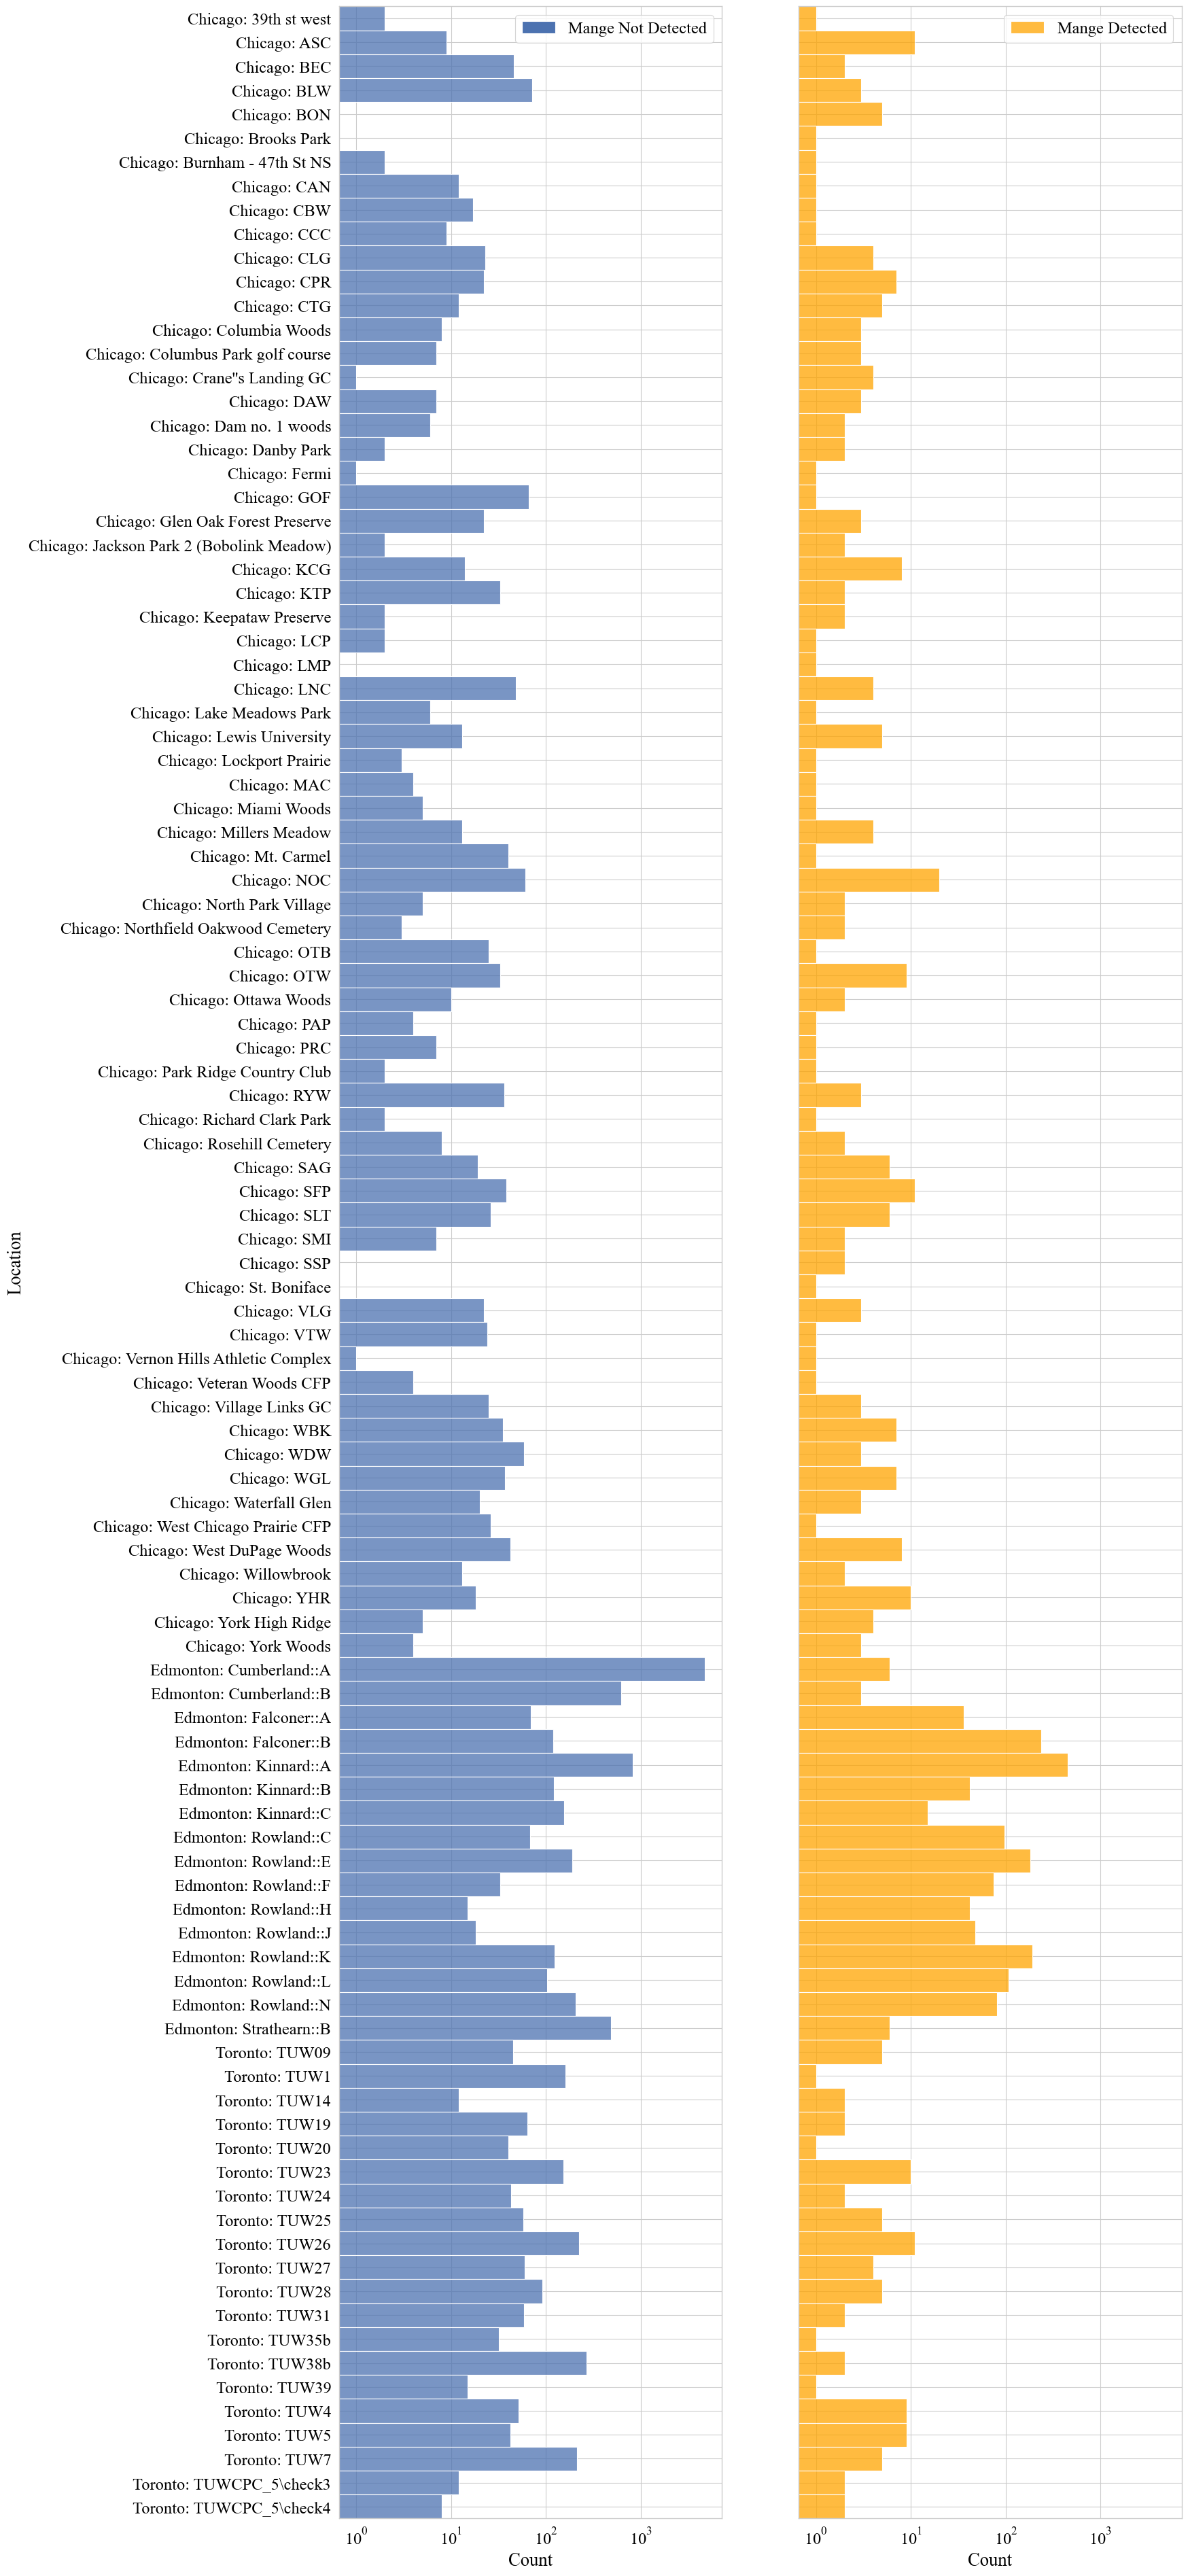
\includegraphics[height=20cm]{fig5.png}
\caption{\label{fig:output}Distribution of our data by location. The horizontal axis represents the log count of images, and the vertical axis lists the locations with at least one sample of "mange detected". There are data distribution differences between locations.}
\end{figure}

\subsection{Integrated Gradients}
With image classification, a key method of understanding the model's learning process is considering which parts of the image the model weighs more heavily in its classification decision. We use one such approach called Integrated Gradients \cite{sundararajan:2017}, which produces an attribution map indicating which parts of the image contribute the most to the classification decision. \\

When applied to our model, we found very different visuals depending on which cross-validation folds it was trained on. This figure depicts the same model trained on two different sets of 5-fold cross-validation folds. Despite sharing $\frac{3}{4}$ folds in their training, the two models focus on very different parts of the same image. The image was excluded from the training sets of both models. This disparity lead us to conclude our location-based separation of data into folds yielded some resulted in variation in training performance on each fold.

\begin{figure}[H]
\centering
\vspace{0cm}
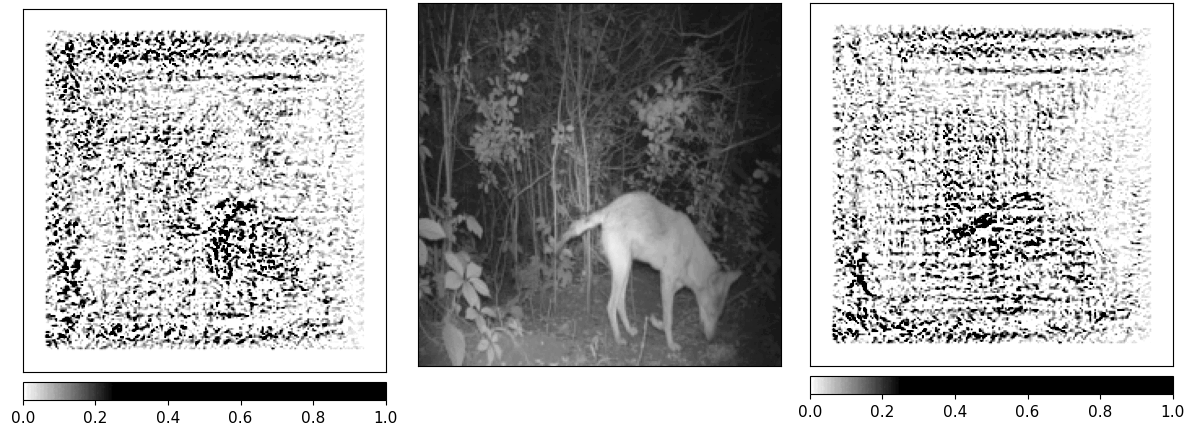
\includegraphics[width=1.0\textwidth]{fig6.png}
\caption{\label{fig:integrated}Integrated gradients applied to the same image using 2 sets of partially intersecting training sets. Left shows more focus on the background, while the right clearly shows focus on the tail.}
\end{figure}

\end{document}